\documentclass{IOS-Book-Article}
\usepackage{amssymb}
\usepackage{array}

\usepackage{graphics}
\usepackage{graphicx}
\usepackage{indentfirst}
\usepackage{enumerate}
\usepackage{listings}
\usepackage{color}
\usepackage{tabularx}
\usepackage{supertabular}
\usepackage{longtable}
\usepackage{natbib}
\usepackage{enumerate}
\usepackage{changepage}
\usepackage{enumitem}
\setenumerate[1]{itemsep=0pt,partopsep=0pt,parsep=\parskip,topsep=0pt}
\setitemize[1]{itemsep=0pt,partopsep=0pt,parsep=\parskip,topsep=0pt}

%for images
\usepackage{tikz}
\usetikzlibrary{positioning,shapes,arrows,arrows.meta,decorations.markings}

\DeclareFixedFont{\mf}{T1}{cmbr}{m}{n}{10pt}

\lstset{ %
  language=Octave,                 % the language of the code
  basicstyle=\tiny,            % the size of the fonts that are used for the code
 %numbers=left,                    % where to put the line-numbers
 %numberstyle=\tiny\color{gray},   % the style that is used for the line-numbers
  stepnumber=2,                    % the step between two line-numbers. If it's 1,  each line 
                                  % will be numbered
  numbersep=5pt,                   % how far the line-numbers are from the code
  backgroundcolor=\color{white},       % choose the background color. You must add \usepackage{color}
  showspaces=false,                % show spaces adding particular underscores
  showstringspaces=false,          % underline spaces within strings
  showtabs=false,                  % show tabs within strings adding particular underscores
  frame=single,                    % adds a frame around the code
  rulecolor=\color{black},         % if not set,  the frame-color may be changed on line-breaks within not-black text (e.g. commens (green here))
  tabsize=2,                       % sets default tabsize to 2 spaces
  captionpos=b,                    % sets the caption-position to bottom
  breaklines=true,                 % sets automatic line breaking
  breakatwhitespace=false,         % sets if automatic breaks should only happen at whitespace
  title=\lstname,                    % show the filename of files included with \lstinputlisting;
                                  % also try caption instead of title
%  keywordstyle=\color{blue},           % keyword style
%  commentstyle=\color{dkgreen},        % comment style
 % stringstyle=\color{mauve},          % string literal style
  escapeinside={\%*}{*)},             % if you want to add LaTeX within your code
  morekeywords={*, ...}               % if you want to add more keywords to the set
}





\begin{document}

\pagestyle{headings}
\def\thepage{}

\begin{frontmatter} 

\title{Checking the validity of rule-based arguments grounded in cases: \\a computational approach}

%\markboth{}{September 2018\hb}
%\subtitle{Subtitle}

\author[A]{\fnms{Heng} \snm{Zheng}\thanks{Corresponding Author: zhengh48@mail2.sysu.edu.cn.}}, \author[B]{\fnms{Minghui} \snm{Xiong}} and \author[A]{\fnms{Bart} \snm{Verheij}}

\runningauthor{H. Zheng et al.}
\address[A]{Artificial Intelligence, University of Groningen, The Netherlands}
\address[B]{Institute of Logic and Cognition, Sun Yat-sen University, Guangzhou, China}

\begin{abstract}
One puzzle studied in AI \& Law is how arguments, rules and cases are formally connected. Recently a formal theory was proposed formalizing how the validity of arguments based on rules can be grounded in cases. Three kinds of argument validity were distinguished: coherence, presumptive validity and conclusiveness. In this paper the theory is implemented in a Prolog program, used to evaluate a previously developed model of Dutch tort law. We also test the theory and its implementation with a new case study modeling Chinese copyright infringement law. In this way we illustrate that by the use of the implementation the process of modeling becomes more efficient and less error-prone.
\end{abstract}

\begin{keyword}
Artificial Intelligence and Law\sep Rule-based Reasoning\sep Case-based Reasoning\sep Argumentation Modeling\sep Prolog
\end{keyword}
\end{frontmatter}
%\markboth{September 2018\hb}{September 2018\hb}

\section{Introduction}
\noindent 
The recent case model formalism \citep{Verheij2016Correct} is a hybrid theory showing connections between cases, rules and arguments~\citep{Verheij2017Formalizing}. The formalism defines different ways in which rule-based arguments can be valid in cases: arguments can be coherent, conclusive or presumptive. The formalism has been applied to model Dutch tort law, showing how a rule-based legal domain can be grounded in legal cases. In this way, a formal connection is established between the civil law tradition focusing on rules and the common law tradition focusing on cases. 

The present paper provides a computational version of the case model formalism. A Prolog program is presented that can computationally check whether a case model is correct, whether rule-based arguments are valid (in the three kinds of validity coherence, conclusiveness and presumptiveness), and whether defeating circumstances are rebutting, undercutting or undermining. The computational tool can be used to support the manual modeling of a complex legal domain, making that more manageable. As an example, we provide a new domain model, namely Chinese copyright infringement law, both formally (as a case model) and computationally (in Prolog).

\section{The implementation of case model formalism in Prolog with case studies}
\label{sec:cm}

\noindent We have implemented the case model formalism in Prolog. We use the previously developed model of Dutch tort law~\cite{Verheij2017Formalizing} as an illustration. Cases are represented as Prolog lists, of which the elements consist of strings and their negations (represented using {\mf not/1}). Case models are represented as lists of cases and their ordering, where case models and cases are referred to using identifiers. 
	\begin{lstlisting}[caption={Definition of the Dutch tort law case model in Prolog},captionpos=b,float]
	case(model_num(1),case_num(101),[not(dmg)]).
	...
	case(model_num(1),case_num(104),[not(dut),dmg,unl,imp,not(cau)]).
	case(model_num(1),case_num(105),[dut,dmg,unl,imp,cau,vrt,not(vst),not(vun),ift,not(ila),not(ico),not(jus),prp]).
	...
	case(model_num(1),case_num(114),[not(dut),dmg,not(unl),vrt,not(vst),jus]).
	...
	case_order(model_num(1),[case_num(101),case_num(102),case_num(103),case_num(104),[case_num(105),case_num(106),...,case_num(113)],...]).
	\end{lstlisting}

Listing 1 provides a part of the representation of the case model for Dutch tort law ({\mf model\_num(1)}). The full model consists of the 16 cases discussed in~\cite{Verheij2017Formalizing}. The ordering is represented as a list of cases and lists of cases, each representing an equivalence class of the total preorder, in decreasing level of preference. Hence the first element of this list represents the case or cases that are maximal in the total preorder. Here there is one maximal case {\mf case\_num(101): not(dmg)}, representing that there are no damages. When an equivalence class consists of several cases, such as {\mf [case\_num(105),...,case\_num(113)]}, it is represented as a list of cases (actually: of case identifiers).

The predicate {\mf case\_model\_valid/1} (with a case identifier as single argument) checks whether all cases are consistent, incompatible and different. Checking whether the ordering of cases is total and transitive is not directly represented since we use an explicit representation of the total preorder as a list of equivalence classes. In this representation another validity check is helpful, namely whether each case of which an identifier appears in the ordering is defined and whether each case identifier of a defined case appears in the ordering exactly once. This check has been implemented using the predicate {\mf ordering\_valid/1}.

Arguments are represented by a list of premises and a list of conclusions. The three kinds of validity of arguments can be checked using the predicates {\mf coherent/1}, {\mf conclusive/1} and {\mf presumptively\_valid/1}, each taking an argument (represented using {\mf argument/2}) as input. Coherence is checked by first determining the case made by an argument, found by appending the list of premises to the list of conclusions, and then checking whether there is a case in the case model that contains all elements of the case made by the argument. 

The conclusiveness of an argument is checked by first checking whether the argument is coherent and then checking, if all cases in the case model that contain the argument's premises also contain its conclusions. 

An argument's presumptive validity is checked by determining a maximally preferred case that witnesses the argument's coherence (i.e., finding a case in which both the premises and conclusions of the argument hold and that is maximal in the ordering with this property) and then checking for each case in which the argument's premises hold whether that case is of equal or lower ordering. 

Attack of arguments has been implemented using the predicates {\mf successful\_attack/2}, {\mf rebutting\_attack/2}, {\mf undercutting\_attack/2} and {\mf undermining\_attack/2}. The predicate {\mf successful\_attack/2} takes an argument and defeating circumstances (as a list) as input. The predicate checks whether the argument is presumptively valid and whether the argument to the same conclusions but from the premises with the defeating circumstances appended is not presumptively valid. 

The three kinds of attack---rebutting, undercutting and undermining---are defined in terms of successful attack as follows. Rebutting attack requires a successful attack of an argument such that also the argument from the premises to the opposite of the argument's conclusion is presumptively valid. Note that this only makes sense for arguments with a single element as conclusion as we use no Prolog expression for the negation of a series of conclusions. Successful attacks that are not rebutting attacks are undercutting. Undermining attack is a special kind of successful attack, namely an attack of an argument with a tautology as premise. In the program, a tautology is represented as an empty Prolog list {\mf [ ]}.

The Prolog program can be used to validate hand-made domain models, such as the case model for Dutch tort law of~\cite{Verheij2017Formalizing}. In Figure~\ref{fig:tort}, we show the argument structure that is valid in the hand-made formal case model of that paper (left). On the right, we show Prolog clauses that all evaluate to true given the Prolog version of that case model (partially shown in Listing 1). In other words, the model is computationally validated.
\newline

\begin{figure*}[btp]
	%\centering
	\scalebox{0.6}{	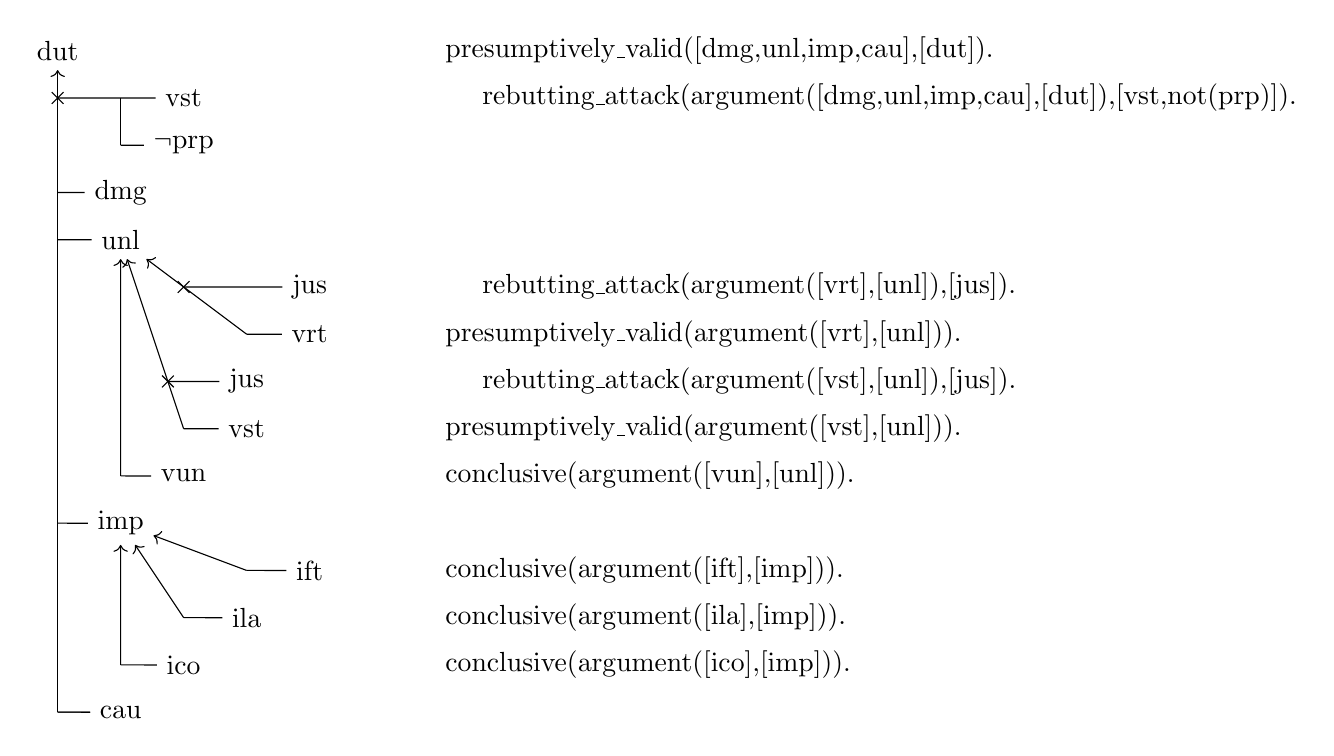
\begin{tikzpicture}	[every text node part/.style={align=center},
		arg/.style={
%			draw,
			%rectangle,
			%-{Straight Barb[angle=60:6pt 0]}
		},
		attack/.style={
			-{Rays[sep=-2.25pt,width=6pt,length=6pt]}
		}
	]

		\begin{scope}
		
		\pgftransformxscale{0.8}
		\pgftransformyscale{0.6}


			\node[arg] (s1) at (0,0) {dut};
			\node[arg] (s2) at (2,-1) {vst};
			\node[arg] (s3) at (2,-2) {$\neg$prp};
			\node[arg] (s4) at (1,-3) {dmg};
			\node[] (s5) at (1,-4) {unl};
%				\draw[] (0.65,-3.75) rectangle (3.5,-4.25);
			\node[arg] (s6) at (4,-5) {jus};
			\node[arg] (s7) at (4,-6) {vrt};
			\node[arg] (s8) at (3,-7) {jus};
			\node[arg] (s9) at (3,-8) {vst};
			\node[arg] (s10) at (2,-9) {vun};
			\node[] (s11) at (1,-10) {imp};
%				\draw[] (0.65,-9.75) rectangle (3.5,-10.25);
			\node[arg] (s12) at (4,-11) {ift};
			\node[arg] (s13) at (3,-12) {ila};
			\node[arg] (s14) at (2,-13) {ico};
			\node[arg] (s15) at (1,-14) {cau};

		\draw[->, arg] (0, -14) -- (s1);
		\draw[] (0, -14) -- (s15);
		\draw[] (0, -3) -- (s4);
		\draw[] (0, -4) -- (s5);
		\draw[] (0, -10) -- (s11);
		\draw[] (0, -14) -- (s15);

		\draw[attack] (s2) -- (0,-1);
		\draw[] (s3) -- (1,-2);
		\draw[] (1,-1) -- (1,-2);

		%\draw[arg] (1, -9) -- (1,-4.25);
		%\draw[arg] (2, -8) -- (2,-4.25);
		%\draw[arg] (3, -6) -- (3,-4.25);
		\draw[->, arg] (1, -9) -- (s5);
		\draw[->, arg] (2, -8) -- (s5);
		\draw[->, arg] (3, -6) -- (s5);
		\draw[] (1, -9) -- (s10);
		\draw[] (2, -8) -- (s9);
		\draw[] (3, -6) -- (s7);

		\draw[attack] (s8) -- (1.75,-7);
		\draw[attack] (s6) -- (2,-5);

		%\draw[arg] (1, -13) -- (1,-10.25);
		%\draw[arg] (2, -12) -- (2,-10.25);
		%\draw[arg] (3, -11) -- (3,-10.25);
		\draw[->, arg] (1, -13) -- (s11);
		\draw[->, arg] (2, -12) -- (s11);
		\draw[->, arg] (3, -11) -- (s11);
		\draw[] (1, -13) -- (s14);
		\draw[] (2, -12) -- (s13);
		\draw[] (3, -11) -- (s12);

		\node[right] at (6,0) {{\mf presumptively\_valid([dmg,unl,imp,cau],[dut]).}};
		\node[right] at (6,-1) {~~~~{\mf rebutting\_attack(argument([dmg,unl,imp,cau],[dut]),[vst,not(prp)]).}};

		\node[right] at (6,-6) {{\mf presumptively\_valid(argument([vrt],[unl])).}};
			\node[right] at (6,-5) {~~~~{\mf rebutting\_attack(argument([vrt],[unl]),[jus]).}};
		\node[right] at (6,-8) {{\mf presumptively\_valid(argument([vst],[unl])).}};
			\node[right] at (6,-7) {~~~~{\mf rebutting\_attack(argument([vst],[unl]),[jus]).}};
		\node[right] at (6,-9) {{\mf conclusive(argument([vun],[unl])).}};
		\node[right] at (6,-11) {{\mf conclusive(argument([ift],[imp])).}};
		\node[right] at (6,-12) {{\mf conclusive(argument([ila],[imp])).}};
		\node[right] at (6,-13) {{\mf conclusive(argument([ico],[imp])).}};



		\end{scope}

	\end{tikzpicture}
}
\caption{The Dutch tort law model: argument structure (left); in Prolog (right)}
\label{fig:tort}
\end{figure*}


%\section{Case study: Copyright infringement in Chinese Criminal Law}
\noindent Another case study is about Chinese copyright infringement. The article of Copyright Infringement in Chinese Criminal Law~\cite{NPC1997CCL} is below:
\newline

\footnotesize
\begin{adjustwidth}{0.5cm}{0cm}
\noindent \textbf{Article 217} Whoever, for the purpose of making profits, commits any of the following acts of infringement on copyright shall, if the amount of illegal gains is relatively large, or if there are other serious circumstances, be sentenced to fixed-term imprisonment of not more than three years or criminal detention and shall also, or shall only, be fined; if the amount of illegal gains is huge or if there are other especially serious circumstances, he shall be sentenced to fixed-term imprisonment of not less than three years but not more than seven years and shall also be fined:

\noindent (1) reproducing and distributing a written work, musical work, motion picture, television programme or other visual works, computer software or other works without permission of the copyright owner;

\noindent (2) publishing a book of which the exclusive right of publication is enjoyed by another person;

\noindent (3) reproducing and distributing an audio or video recording produced by another person without permission of the producer; or

\noindent (4) producing or selling a work of fine art with forged signature of another painter.\newline
\end{adjustwidth}

\normalsize
\noindent 
According to the articles related to Art. 217 in Chinese criminal law~\cite{NPC1997CCL}, and relevant official judicial interpretations~\cite{SupremeCourt2011Judicial}, there is a defeating circumstance: the action was not belong to ``without permission of the copyright owner".


\begin{table}[b]
	\tiny
	\caption{Elementary propositions in the copyright infringement model with abbreviations}
	\label{tab:abbr}
	\begin{tabularx}{\textwidth}{p{0.5cm}|p{11cm}}
		\hline
		ifg & there is a copyright infringement\\
		fpp & the act was for the purpose of making profits\\
		rad & the act was reproducing and distributing something\\
		ite & the act concerned the items in Art. 217:1\\
		pco & the act was without permission of the copyright owner\\
		npo & the act was not belong to "without permission of the copyright owner"\\
		epr & a book is published of which the exclusive right of publication is enjoyed by another person\\
		avp & a audio or video recording is produced by another person without permission of the producer\\
		psa & a work of fine art with forged signature of another painter is produced or sold\\
		ils & the amount of illegal gains is large or other serious circumstances\\
		ihe & the amount of illegal gains is huge or other especially serious circumstances\\
		crc & the person commits the crime of copyright infringement\\
		l3fti & the person shall be sentenced to fixed-term imprisonment of at most three years\\
		cdt & the person shall be sentenced to criminal detention\\
		fin & the person shall be fined\\
		m3fti & the person shall be sentenced to fixed-term imprisonment of not less than three years but not more than seven years\\
		cpb & the defendant satisfies the conditions of probation\\
		pbt & the defendant will be put on probation\\
		\hline
	\end{tabularx}
\end{table}
\begin{table}[b]
	\tiny
	\caption{The Chinese copyright infringement case model (selection)}
	\label{tab:long}
	\begin{tabularx}{\textwidth}{p{1.2cm}|p{10cm}}
		\hline
		Case 1 & $\neg$rad,$\neg$ite,$\neg$pco,$\neg$epr,$\neg$avp,$\neg$psa,$\neg$ifg\\
		Case 2 & rad,ite,pco,npo,$\neg$ifg\\
		Case 3 & rad,ite,pco,$\neg$npo,$\neg$epr,$\neg$avp,$\neg$psa,ifg,$\neg$fpp\\
		Case 4 & rad,ite,pco,$\neg$epr,$\neg$avp,$\neg$psa,ifg,fpp,ihe,$\neg$ils,crc,m3fti,$\neg$l3fti,$\neg$cdt,fin\\
		Case 5 & rad,ite,pco,$\neg$epr,$\neg$avp,$\neg$psa,ifg,fpp,$\neg$ihe,ils,crc,$\neg$m3fti,$\neg$l3fti,$\neg$cdt,fin\\
		Case 6 & rad,ite,pco,$\neg$epr,$\neg$avp,$\neg$psa,ifg,fpp,$\neg$ihe,ils,crc,$\neg$m3fti,l3fti,$\neg$cdt,fin,cpb,pbt\\
		Case 7 & rad,ite,pco,$\neg$epr,$\neg$avp,$\neg$psa,ifg,fpp,$\neg$ihe,ils,crc,$\neg$m3fti,$\neg$l3fti,cdt,fin,cpb,pbt\\
		Case 8 & rad,ite,pco,$\neg$epr,$\neg$avp,$\neg$psa,ifg,fpp,$\neg$ihe,ils,crc,$\neg$m3fti,l3fti,$\neg$cdt,fin,$\neg$cpb,$\neg$pbt\\
		Case 9 & rad,ite,pco,$\neg$epr,$\neg$avp,$\neg$psa,ifg,fpp,$\neg$ihe,ils,crc,$\neg$m3fti,$\neg$l3fti,cdt,fin,$\neg$cpb,$\neg$pbt\\					... & ...\\
		\hline
	Case order & Case 1 $>$ Case 2 = Case 3 $>$ Case 4 = Case 5 = Case 6 = Case 7 = Case 8 = Case 9\\
	\hline
	\end{tabularx}
\end{table}

\normalsize

In the light of Art. 217 and the judicial interpretations related to it, a case model based on Verheij's case model formalism with a similar modeling approach to the Dutch tort law model in~\cite{Verheij2017Formalizing} can be built. We use the elementary propositions in Table~1, shown with their formal abbreviations. 
The full model has 30 cases. A selection of the cases is shown in its case list version in Table~2. The model has identifier {\mf model\_num(2)}. 
In the text below, cases are numbered 1, 2, 3, ... corresponding  to cases {\mf 201, 202, 203, ...} in the Prolog version.

\normalsize

\begin{figure*}[t]
	\scalebox{0.6}{	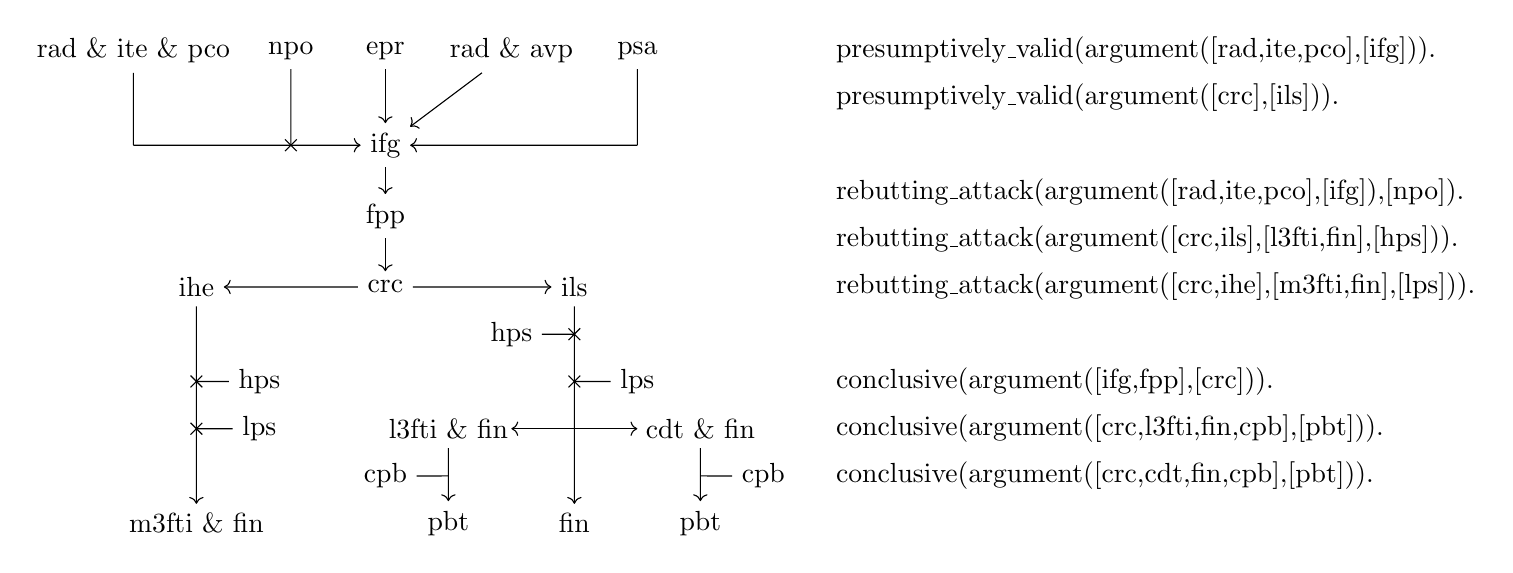
\begin{tikzpicture}	[every text node part/.style={align=center},
		arg/.style={
%			draw,
			%rectangle,
			%-{Straight Barb[angle=60:6pt 0]}
		},
		attack/.style={
			-{Rays[sep=-2.25pt,width=6pt,length=6pt]}
		}
	]

		\begin{scope}
		
		\pgftransformxscale{0.8}
		\pgftransformyscale{0.6}

			\node[arg] (s1) at (0,1) {epr};
			\node[arg] (s2) at (-1.5,1) {npo};
			\node[arg] (s3) at (-4,1) {rad \& ite \& pco};
			\node[arg] (s4) at (2,1) {rad \& avp};
			\node[arg] (s5) at (4,1) {psa};
			\node[arg] (s6) at (0,-1) {ifg};
			\node[arg] (s7) at (0,-2.5) {fpp};
			\node[arg] (s8) at (0,-4) {crc};
			\node[arg] (s9) at (2,-5) {hps};
			\node[arg] (s10) at (4,-6) {lps};
			\node[arg] (s11) at (-3,-4) {ihe};
			\node[arg] (s12) at (3,-4) {ils};
			\node[arg] (s13) at (-2,-6) {hps};
			\node[arg] (s15) at (-2,-7) {lps};
			\node[arg] (s16) at (1,-7) {l3fti \& fin};
			\node[arg] (s18) at (5,-7) {cdt \& fin};
			\node[arg] (s19) at (0,-8) {cpb};
			\node[arg] (s20) at (3,-9) {fin};
			\node[arg] (s21) at (6,-8) {cpb};
			\node[arg] (s22) at (-3,-9) {m3fti \& fin};
			\node[arg] (s23) at (1,-9) {pbt};
			\node[arg] (s24) at (5,-9) {pbt};


		\draw[] (s3) -- (-4,-1);
		\draw[->] (-4,-1) -- (s6);
		\draw[attack] (s2) -- (-1.5,-1);
		\draw[] (s5) -- (4,-1);
		\draw[->] (4,-1) -- (s6);
		\draw[attack] (s13) -- (-3, -6);
		\draw[attack] (s15) -- (-3, -7);
		\draw[->] (3,-7) -- (2,-7);
		\draw[->] (3,-7) -- (4,-7);
		\draw[] (s19) -- (1,-8);
		\draw[] (s21) -- (5,-8);
		\draw[attack] (s9) -- (3, -5);
		\draw[attack] (s10) -- (3, -6);
		\draw[->, arg] (s1) -- (s6);
		\draw[->, arg] (s4) -- (s6);
		\draw[->, arg] (s6) -- (s7);
		\draw[->, arg] (s7) -- (s8);
		\draw[->, arg] (s8) -- (s11);
		\draw[->, arg] (s8) -- (s12);
		\draw[->, arg] (s11) -- (s22);
		\draw[->, arg] (s12) -- (s20);
		\draw[->, arg] (s16) -- (s23);
		\draw[->, arg] (s18) -- (s24);

		
	\node[right] at (7,1) {{\mf presumptively\_valid(argument([rad,ite,pco],[ifg])).}};
	\node[right] at (7,0) {{\mf presumptively\_valid(argument([crc],[ils])).}};
	\node[right] at (7,-2) {{\mf rebutting\_attack(argument([rad,ite,pco],[ifg]),[npo]).}};
	\node[right] at (7,-3) {{\mf rebutting\_attack(argument([crc,ils],[l3fti,fin],[hps])).}};
	\node[right] at (7,-4) {{\mf rebutting\_attack(argument([crc,ihe],[m3fti,fin],[lps])).}};
	\node[right] at (7,-6) {{\mf conclusive(argument([ifg,fpp],[crc])).}};
	\node[right] at (7,-7) {{\mf conclusive(argument([crc,l3fti,fin,cpb],[pbt])).}};
	\node[right] at (7,-8) {{\mf conclusive(argument([crc,cdt,fin,cpb],[pbt])).}};
	

		\end{scope}

	\end{tikzpicture}
}
\caption{The Chinese copyright infringement model: argument structure (left); in Prolog (right)}
\label{fig:copyright}
\end{figure*}


From Chinese copyright infringement, we can analyze the argument structure as in the diagram in Figure~\ref{fig:copyright} (left). This argument structure shows multiple rule-based steps and an exception-based attack. The structure is valid in the case model we built. Following the definitions of the case model formalism, the  arguments in Figure 2 (right) can be extracted in the model. The Prolog program confirms the validity of these arguments. These Prolog queries are evaluated as true, which means the results of the Prolog program correspond to our analysis of the Chinese copyright infringement model.

\section{Conclusion}

\noindent 
The results of this paper show that an implementation of the case model formalism can be used to support the modeling of a legal domain with a complex argument structure involving combined support and attack\footnote{The full program code and the Chinese copyright infringement model are available at https://github.com/Zhe333/Appendix.git}. In this way, we have shown a computational connection between cases, rules and arguments, applied to the civil law system of the Netherlands and to criminal law in the Chinese legal system. AI and legal reasoning technology needs to combine rule-based reasoning, case-based reasoning and argumentation together, paving the way for argumentation technology that bridges cases and rules, as it is common in the law.

\footnotesize
\bibliographystyle{unsrt}
\setcitestyle{round,aysep={},yysep={;}}
\bibliography{AIandLaw}


\end{document}